\chapter{Validation et détails d'implémentation}

\section{Vue d'ensemble de la solution proposée}

Comme on le voit \ref{archi}

\begin{wrapfigure}{r}{.7\textwidth}
    \centering
    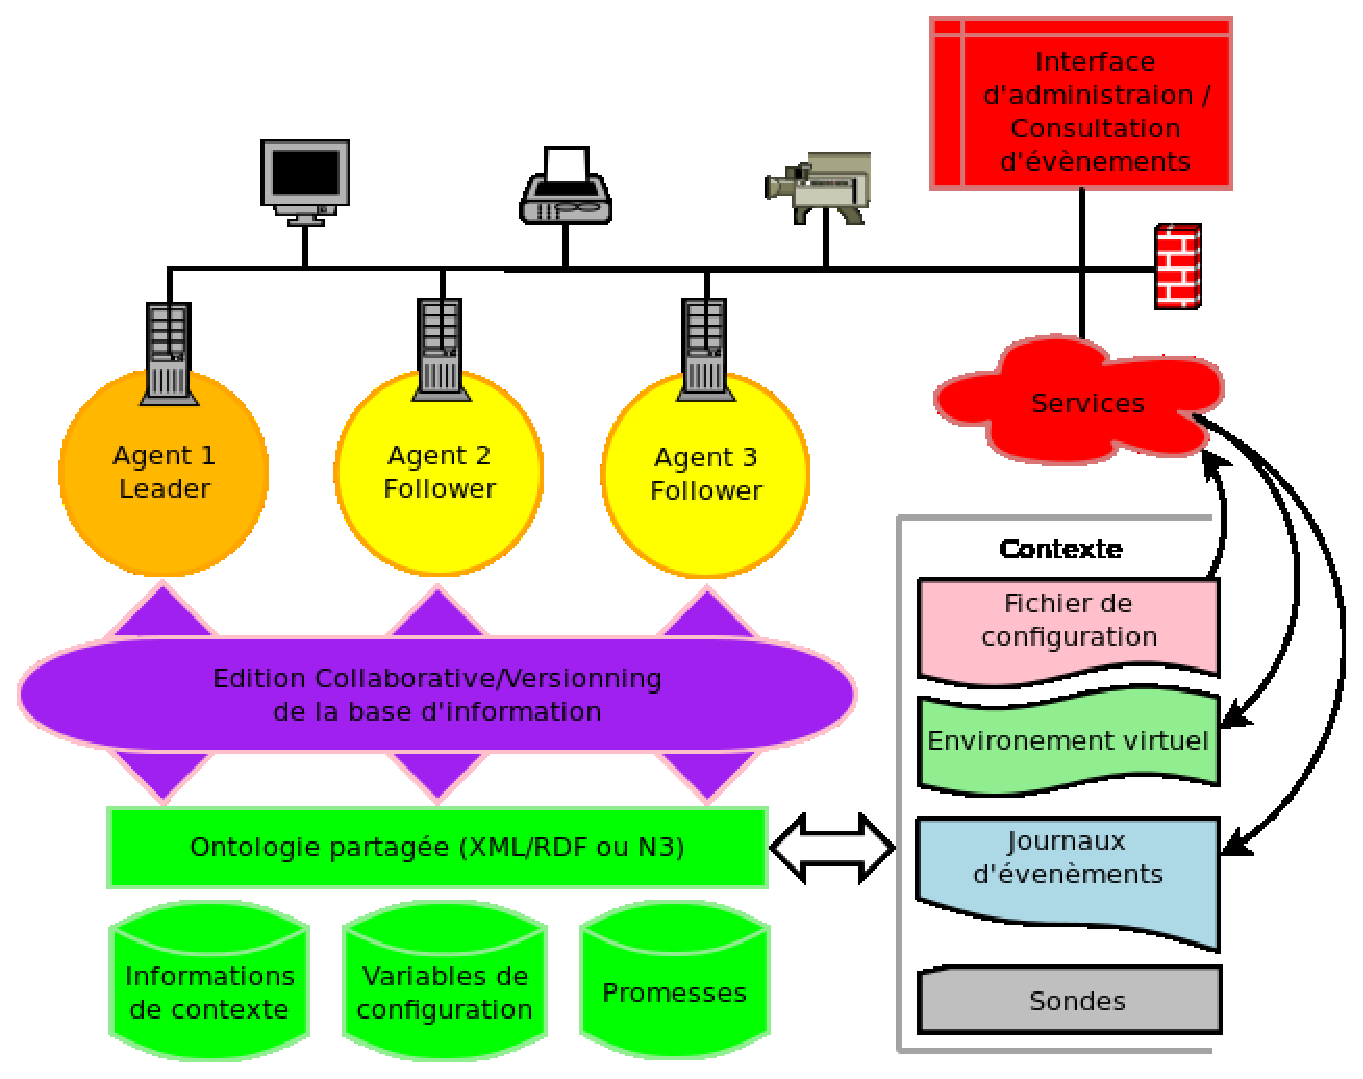
\includegraphics[width=.67\textwidth]{img/archi}
    \caption{Schéma d'implémentation du système multi-agents}
    \label{archi}
\end{wrapfigure}

\section{Framework de gestion de configuration}

La gestion de la configuration est le processus de contraindre le comportement
d'un réseau de machines de manière à ce que le comportement de chaque machine
soit conforme aux politiques et lignes directrices prédéfinies, et
accomplisse les objectifs d'entreprise prédéterminés. Cela implique :

\begin{itemize}
  \item Des personnes
  \item Outil gestion de configuration ``zéro`` (exemple: CfEngine)
  \item Un ensemble ce machines interconnectées
  \item Un ensemble de processus de configuration destiné à aboutir à un système
	  conforme à la politique en vigueur.
\end{itemize}

Les paramètres de configuration peuvent être la permission d'un fichier,
l'adresse d'un carte réseau, le type de système de fichier pouvant être monté
sur un volume disque.

La possibilité d'automatiser la configuration des réseaux IP (Internet
Protocol) en utilisant une technologie sémantique est également très
prometteuse. L'initiative connexe de créer un environnement de réseau de
capteurs basé sur le ontologies semble également être une solution viable.

La plupart des organisations aujourd'hui n'ont aucun procédé systématique pour
gérer leurs informations de configuration. Cela signifie que des informations
comme l'adresse IP d'une machine et le statut de son service réseau sont
stockées de manière dispersée et désorganisée. Certains outils de supervision
tels que Nagios présente une manière de réorganiser ces informations provenant
de sources dispersées.

L'idée d'utiliser une CMDB (Configuration Management Database) est également un
alternative permettant de solutionner le problème ci-dessus. Toutefois, le besoin
pour un gestionnaire d'informations de plus haut niveau est mentionné dans de
nombreuses littératures.

Cette nouvelle façon de renforcer l'efficacité de la gestion des connaissances
dans le domaine de la gestion de configuration, nécessite la possibilité
d'extraction automatique de données à partir d'emplacements de stockage
précédents et la possibilité de mise à jour automatique de stockages permanents
tels que la CMDB afin d'augmenter la qualité de l'information sous-jacente.

La possibilité de ces deux fonctions à savoir, l'extraction automatique des
données et également la mise à jour automatique des informations stockées ont
été fournies par ITIL. % FIXME ITIL ?

Le travail de ce mémoire est de démontrer les possibilités d'obtenir un
gestionnaire de connaissances intégré en conjuguant les ontologies, la théorie
de la promesse et le consensus de Raft. La structure de l'information de
configuration stockée dans une CMDB et dans d'autres fichiers sera représentée en
concordance avec les standard de OWL. Cette structure de domaine de connaissance
sera implémentée comme une promesse de structure d'information.

\noindent\rule{8cm}{0.4pt}

La Configuration Management Database (abrégé CMDB), ou base de données de
gestion de configuration, est une base de données unifiant les composants d'un
système informatique. Elle permet de comprendre l'organisation entre ceux-ci et
de modifier leur configuration. La CMDB est un composant fondamental d'une
architecture ITIL.

\section{Gestionnaire de configuration basé sur la théorie de la promesse}

\subsection{Ontologie de contexte}

La structure de base de l'ontologie de contexte a été implémentée à l'aide du
logiciel libre \emph{Protégé}. Elle met a disposition une définition générique
des composants les plus standard d'un réseau d'application comme les interfaces,
les processus, les utilisateurs ou encore les fichiers et leurs permissions
associées. Le détail des entités de cette ontologie sont données en
annexe \ref{appendix:ontology}. La structure n'est pas figée, elle apporte
seulement la pierre angulaire pour la définition de nouveaux concepts plus
spécifiques. En effet, la structure s'étend à mesure à des sondes sont ajoutées.
Celle-ci formalisent un certain nombre d'informations de manière individuelle et
la structure découle alors de la mise en corrélation de ces informations.

\subsection{Sondes de contexte}

\begin{wrapfigure}{r}{.5\textwidth}
  \begin{alltt}\scriptsize
    \textbf{user1@server1\$} trifle console

    store   = Store()  # 10598 statements
    server1 = Server() # uuid: d7c38143d6ed41c8ad1f04c9601733d1)
    server2 = Server() # uuid: 4a1950ded8c141dd91b695e6f6a09f07)
    
    >>> store
    <trifle.store.Store instance at 0x336acf8>
    >>> len(store.graph)
    10598
    >>> store.snapshot()
    2014-08-14 15:08:07 \textbf{INFO} Pulling from InterfacesSensor...
    2014-08-14 15:08:07 \textbf{DEBUG} 36 informations sensored
    2014-08-14 15:08:07 \textbf{INFO} Pulling from ProcessesSensor...
    2014-08-14 15:08:08 \textbf{WARNING} NoSuchProcess: 24963
    2014-08-14 15:08:08 \textbf{WARNING} NoSuchProcess: 24964
    2014-08-14 15:08:08 \textbf{WARNING} NoSuchProcess: 25080
    2014-08-14 15:08:08 \textbf{WARNING} NoSuchProcess: 25082
    2014-08-14 15:08:08 \textbf{DEBUG} 1395 informations sensored
    2014-08-14 15:08:09 \textbf{INFO} Pulling from UsersSensor...
    2014-08-14 15:08:09 \textbf{DEBUG} 15 informations sensored
    [...]
    >>> len(store.graph)
    14534
  \end{alltt}
  \caption{Capture et fusion des informations de contexte provenant des sondes}
  \label{fig:sensor}
\end{wrapfigure}

Afin de garantir la flexibilité et l'extensibilité de notre gestionnaire, les
sondes de contextes sont implémentées sous la forme d'un greffon. Une classe
\emph{BaseSensor} est mise à disposition à titre de manifeste pour la création
de nouvelles sondes. L'interface implémente la méthode \emph{pull()} permettant
la population de l'ontologie de contexte.

Le processus de fusion des information est assez simple dans l'implémentation
puisqu'elle prend avantage des méthodes de manipulation de graphes intégrées à
la librairie Python RDFlib. Il ne peut exister ni d'informations redondantes, ni
de relations dépourvues d'acteurs : l'information demeure consistante.

Chacune de ces sondes va permettre de recueillir les informations relatives au
contexte local, c.a.d, les informations liées à la machine sur laquelle opère
l'agent. Lors de l'incrémentation d'un terme dans le cycle de fonctionnement
normal basé sur le consensus de Raft, les informations recueillies par chacun
des agents seront misent en corrélation. La méthode \emph{snapshot()} autorise
par ailleurs le renouvellement complet de la base d'informations.  La figure
\ref{fig:sensor} montre (partiellement) le résultat de cette méthode.  Un
information correspond à un triplet $\langle a P b \rangle$, où $b$ est une
valeur de la propriété $P$ pour le sujet $a$. Ne vous laissez pas confondre par
la terminologie : une relation, un prédicat et une propriété sont trois termes
pour la même notion. La relation $\langle a P b \rangle$ utilise le prédicat
$P$, et exprime que le sujet $a$ a une valeur $b$ pour la propriété $P$.

\subsection{Système multi-agents}

\subsubsection{Consensus de Raft}

\begin{wrapfigure}{r}{.5\textwidth}
  \begin{alltt}\scriptsize
    \textbf{user1@server1\$} trifle console

    store   = Store()  # 10598 statements
    server1 = Server() # uuid: d7c38143d6ed41c8ad1f04c9601733d1)
    server2 = Server() # uuid: 4a1950ded8c141dd91b695e6f6a09f07)
    
    >>> server1, server2
    (<Server(Thread-1, started daemon 140389140690688)>, 
     <Server(Thread-2, started daemon 140388924913408)>)
    >>> server1.role, server2.role
    ('follower', 'leader')
    >>> server1.call_election()
    >>> server1.role, server2.role
    ('leader', 'follower')
  \end{alltt}
  \caption{Validation de l'implémentation du consensus de Raft}
  \label{fig:raft}
\end{wrapfigure}

Le mécanismes que décrit le consensus de Raft ont été implémentés en Python.
Dans notre implémentation, on suppose qu'il n'existe qu'un seul agent par
machine. Tout d'abord, parce qu'il n'y a que très peu d'intérêts à déployer
plusieurs instance sur la même machine, et ensuite, parce que cela facilite
grandement le processus de découverte de nouvelles ressources. En effet, le
service (l'agent) sera mis à disposition à travers un port de communication
TCP/UDP figé : 6182 (hormis le fait qu'il n'est actuellement utilisé par aucune
application courante, le choix de ce port est complètement arbitraire). Ainsi,
il sera beaucoup moins coûteux de balayer chacune des plages du réseau à la
recherche de nouveaux agents.

Dans la figure \ref{fig:raft}, le gestionnaire est lancé en mode console. Le
serveur 1 correspond au serveur local et le serveur 2 est un serveur distant. À
l'initialisation du programme, une campagne est lancée et l'un des deux serveur
est élu \emph{leader}. Le \emph{follower} (serveur 2) va supposer une
défaillance du leader (arrêt des pulsations) et donc renouveler la campagne à
laquelle il est \emph{candidat} (et même favori). À l'issue de cette seconde
élection, on remarque que c'est désormais le second serveur qui est à la tête du
système et les opérations ont repris leur cours normal.

\subsubsection{Requêtes}

% TODO Requests

\subsection{Interface d'administration}

Le gestionnaire de configuration prévoit un interface d'administration
pour la définition des politiques de comportement et le contrôle des différents
composants du système. L'interface est un service web distribué par
chacun des agents. Toutes les actions effectuées à travers l'interface seront
opérées par le leader du cluster afin de prévenir les problèmes liés à des
modifications concurrentes. L'ontologie de contexte sera directement
consultable en temps réel à l'aide de requêtes SPARQL. Enfin, elle doit
conserver la possibilité de renseigner les valeurs des variables de
configuration de bas niveau. Des captures d'écran de l'interface
d'administration sont disponibles en annexe \ref{appendix:interface}.

\section{Conclusion}

Les technologies basées sur le contexte vont jouer un rôle fondamental dans la
prochaine génération de systèmes informatiques à mesure que la complexité des
logiciels, la diversité et l'omniprésence des périphériques continuent
d'augmenter. Cependant, elle doivent offrir des mécanismes permettant la
gestion automatique des dépendances inter-composants et composant/ressource.
Dans le cas contraire, le développement de systèmes basés sur les composants
demeura difficile à appréhender et conduira bien souvent à des systèmes peu
fiables et pas assez robustes.

Les environnements qui composeront l'informatique ubiquitaire de demain sera
composé de milliers de périphériques, avec des millions de composantes
logicielles. Les systèmes actuels s'appuient fortement sur la configuration
manuelle, ce qui à un telle échelle n'est plus possible. Il n'existe que deux
issues possible à cette situation : une configuration statique, ou une
configuration dynamique et automatique. Puisque les environnements ont
tendance à être de plus en plus dynamiques, la configuration autonome semble
incarner la seule solution viable.

% ex: set spelllang=fr spell: %
%%% Local Variables: ***
%%% mode: latex ***
%%% TeX-master: "thesis.tex" ***
%%% End: ***
